\section{Subset Sum where $S = W$}
\begin{theorem}{}Subset Sum Reconfiguration is strongly \NP-hard
\end{theorem}

\subsection{Preliminaries}
\begin{itemize}
    \item A packing $A_i$ is the subset of items in a set $A$ such that the total size of $A_i \leq$ capacity $c$ of a knapsack problem.
    \item The size of a packing $A_i = s(A_i)$.
    \item A packing doesn't necessarily satisfy a treshold $k$.
    \item Two packings are adjacent if their symmetric difference is of cardinality $1$.
    \item A reconfiguration sequence $P$ between two packings $A_0$ and $A_t$ is a sequence of packings $A_0, A_1, \dots, A_t$ such that $A_{i-1}$ and $A_i$ are adjacent $\forall i = 1, 2, \dots, t$.
    \item The minimum total size among all packings in $P$ is equal to $f(P)$ where $f(P) = min \{s(A_i) = A_i \in P\}$.
    \item For two packings $A_0$ and $A_t$ : $OPT(A_0, A_t) = max \{ f(P) : P$ is a reconfiguration sequence between $A_0$ and $A_t\}$.
\end{itemize}

\begin{defn}{(Subset Sum Reconfiguration).} Given an integer treshold $k$ and two packings $A_0$ and $A_t$, the Subset Sum reconfiguration problem is to determine whether $OPT(A_0, A_t) \geq k$.
\end{defn}

\begin{proof} $3$-partition problem $\leq_p$ Subset Sum Reconfiguration problem.

\begin{defn}{($3$-partition problem).} Given a positive integer bound $b$, a set $U$ of $3m$ elements $U_1,U_2, \dots, U_{3m}$, each element $u_i \in U$ has a positive size $s(u_i)$ such that $b/4 < s(u_i) < b/2$ and such that $\sum_{u \in U} s(u) = mb$. Then the $3$-partition problem is to determine whether $U$ can be partitioned in $m$ disjoint subsets
$U_1,U_2, \dots, U_{m}$ such that $\sum_{u \in U} s(u) = b$  $\forall j \in 1,\dots, m$.
\end{defn}

\paragraph{Reduction Construction} Given an instance of the $3$-partition problem, we construct the corresponding instance of the SUBSET SUM RECONFIGURATION problem.
\begin{itemize}
    \item From the given set $A$ and bound $b$, we will define a set $A$ consisting of $4m$ elements $a_1, a_2,\dots,a_{3m},b_1,b_2,\dots,b_m$.
    \item Let $s(a_i) = s(u_i)$ for each $i, 1 < i < 3m$. \\ Let $s(b_j) = b $ for each $j, 1 < j < m$. \\ Then each item $a_i$ corresponds to the element $u_i \in U$.
    \item The capacity $c$ will be $c.m$.
    \item The treshold $k = (m-1)b$.
    \item The two packings $A_0$ and $A_t$ are defined as follows :
    \begin{itemize}
        \item $A_0 = \{b_1, b_2,\dots, b_m\}$.
        \item $A_t = U$ \\ Both $A_0$ and $A_t$ are of total size $mb$ satisfying the constraint of the $3-partition$ problem.
    \end{itemize}
\end{itemize}

\paragraph{Correctness} Since $k = (m-1)b$ and $s(b_j) = b \forall j, 1 < j < m$, there exists a desired partition $\{U_1, U_2,\dots,u_m\}$ if and only if there exist a reconfiguration sequence $P$ between $A_0$ and $A_t$ with $f(P) = k = (m-1)b$ and hence $OPT(A_0, A_t) = (m-1)b \geq k$. \todo{Add more explanation to why}
\end{proof}

\begin{example}
    \begin{figure}[H]
        \begin{center}
            \begin{scaletikzpicturetowidth}{\textwidth}
                \begin{tikzpicture}[scale=1]
                    \node (16) [draw, rectangle] {\{\}};
                    \node (1) [right=of 16, draw, rectangle] {\{20\}};
                    \node (2) [below=of 1, draw, rectangle] {\{25\}};
                    \node (3) [below=of 2, draw, rectangle] {\{45\}};
                    \node (4) [label={$A_0$}, below=of 3, draw, rectangle] {\{90\}};
                    \node (5) [above right=of 1, draw, rectangle] {\{20, 25\}};
                    \node (6) [right=of 1, draw, rectangle] {\{20, 45\}};
                    \node (7) [right=of 2, draw, rectangle] {\{20, 90\}};
                    \node (8) [right=of 3, draw, rectangle] {\{25, 45\}};
                    \node (9) [right=of 4, draw, rectangle] {\{25, 90\}};
                    \node (10) [below right=of 4, draw, rectangle] {\{45, 90\}};
                    \node (11) [label={$A_t$},right=of 6, draw, rectangle] {\{20, 25, 45\}};
                    \node (12) [right=of 7, draw, rectangle] {\{20, 25, 90\}};
                    \node (13) [right=of 8, draw, rectangle] {\{20, 45, 90\}};
                    \node (14) [right=of 9, draw, rectangle] {\{25, 45, 90\}};
                    \node (15) [right=of 12, draw, rectangle] {\{20, 25, 45, 90\}};

                    \draw[-, red]  (16) to node [auto] {} (1);
                    \draw[-]  (16) to node [auto] {} (2);
                    \draw[-]  (16) to node [auto] {} (3);
                    \draw[-, red]  (16) to node [auto] {} (4);
                    \draw[-, red]  (1) to node [auto] {} (5);
                    \draw[-]  (1) to node [auto] {} (6);
                    \draw[-]  (1) to node [auto] {} (7);
                    \draw[-]  (2) to node [auto] {} (5);
                    \draw[-]  (2) to node [auto] {} (8);
                    \draw[-]  (2) to node [auto] {} (5);
                    \draw[-]  (3) to node [auto] {} (6);
                    \draw[-]  (3) to node [auto] {} (8);
                    \draw[-]  (3) to node [auto] {} (10);
                    \draw[-]  (4) to node [auto] {} (7);
                    \draw[-]  (4) to node [auto] {} (9);
                    \draw[-]  (4) to node [auto] {} (10);
                    \draw[-, red]  (5) to node [auto] {} (11);
                    \draw[-]  (5) to node [auto] {} (12);
                    \draw[-]  (6) to node [auto] {} (11);
                    \draw[-]  (6) to node [auto] {} (13);
                    \draw[-]  (7) to node [auto] {} (12);
                    \draw[-]  (7) to node [auto] {} (13);
                    \draw[-]  (8) to node [auto] {} (11);
                    \draw[-]  (8) to node [auto] {} (14);
                    \draw[-]  (9) to node [auto] {} (12);
                    \draw[-]  (9) to node [auto] {} (14);
                    \draw[-]  (10) to node [auto] {} (13);
                    \draw[-]  (10) to node [auto] {} (14);
                    \draw[-]  (11) to node [auto] {} (15);
                    \draw[-]  (12) to node [auto] {} (15);
                    \draw[-]  (13) to node [auto] {} (15);
                    \draw[-]  (14) to node [auto] {} (15);
                \end{tikzpicture}
            \end{scaletikzpicturetowidth}
        \end{center}
        \caption{All packings for $A$ = \{20,25,45\} and c = 90}\label{fig:specialCase}
    \end{figure}
\end{example}


\begin{itemize}
    \item $\mathcal{U} = \{v_1, v_2, v_3, v_4, v_5, v_6\} \cup \{t_1, t_2\}.$
    \item The set $\mathcal{S}$ :
    \begin{itemize}
        \item $\{v_1, v_3, v_5, v_6\}, \{v_2, v_3, v_5, v_6\},
        \{v_2, t_1\}, \{v_1, t_1\}, \{v_2, t_2\}, \{v_1, t_2\}, \\
        \{v_1, v_2, v_3, v_5, v_6, t_1\},  \{v_1, v_2, v_3, v_5, v_6, t_2\}$. \textcolor{gray}{$(v_1, v_2)$}

        \item $\{v_1, v_2, v_3, v_4, v_6\}, \{v_2, v_3, v_4, v_5, v_6\},
        \{v_5, t_1\}, \{v_1, t_1\}, \{t_2, v_5\}, \{v_1, t_2\}, \\
        \{v_1, v_2, v_3, v_4, v_5, v_6, t_1\}, \{v_1, v_2, v_3, v_4, v_5, v_6, t_2\}$.  \textcolor{gray}{$(v_1, v_5)$}

        \item $\{v_1, v_2, v_4, v_5\}, \{v_2, v_4, v_5, v_6\},
        \{v_6, t_1\}, \{v_1, t_1\}, \{v_6, t_2\}, \{v_1, t_2\}, \\
        \{v_1, v_2, v_4, v_5, v_6, t_1\}, \{v_1, v_2, v_4, v_5, v_6, t_2\}$.   \textcolor{gray}{$(v_1, v_6)$}

        \item $\{v_1, v_2, v_4, v_5, v_6\}, \{v_1, v_3, v_4, v_5, v_6\},
        \{v_3, t_1\}, \{v_2, t_1\}, \{v_3, t_2\}, \{v_2, t_2\}, \\
        \{v_1, v_2, v_3, v_4, v_5, v_6, t_1\}, \{v_1,v_2,v_3,v_4,v_5,v_6,t_2\}$. \textcolor{gray}{$(v_2, v_3)$}

        \item $\{v_1, v_2, v_3, v_4\}, \{v_1, v_3, v_4, v_6\},
        \{v_6, t_1\}, \{v_2, t_1\}, \{v_6, t_2\}, \{v_2, t_2\}, \\
        \{v_1, v_2, v_3, v_4, v_6, t_1\}, \{v_1, v_2, v_3, v_4, v_6, t_2\}$.   \textcolor{gray}{$(v_2, v_6)$}

        \item $\{v_2, v_3, v_5, v_6\}, \{v_2, v_4, v_5, v_6\},
        \{v_4, t_1\}, \{v_3, t_1\}, \{v_4, t_2\}, \{v_3, t_2\}, \\
        \{v_2, v_3, v_4, v_5, v_6, t_1\}, \{v_2, v_3, v_4, v_5, v_6, t_2\}$.   \textcolor{gray}{$(v_3, v_4)$}

        \item $\{v_1, v_2, v_3, v_4\}, \{v_1, v_2, v_4, v_5\},
        \{v_5, t_1\}, \{v_3, t_1\}, \{v_5, t_2\}, \{v_3, t_2\}, \\
        \{v_1, v_2, v_3, v_4, v_5, t_1\}, \{v_1, v_2, v_3, v_4, v_5, t_2\}$.  \textcolor{gray}{$(v_3, v_5)$}

        \item $\{v_1, v_3, v_4, v_6\}, \{v_1, v_3, v_5, v_6\},
        \{v_5, t_1\}, \{v_4, t_1\}, \{v_5, t_2\}, \{v_4, t_2\}, \\
        \{v_1, v_3, v_4, v_5, v_6, t_1\}, \{v_1, v_3, v_4, v_5, v_6, t_2\}$.  \textcolor{gray}{$(v_4, v_5)$}

        \item $\{v_1, v_2, v_3, v_4, v_5\}, \{v_1, v_2, v_3, v_5, v_6\},
        \{v_6, t_1\}, \{v_4, t_1\},  \{v_6, t_2\}, \{v_4, t_2\}, \\
        \{v_1, v_2, v_3, v_4, v_5, v_6, t_1\}, \{v_1, v_2, v_3, v_4, v_5, v_6, t_2\}$.  \textcolor{gray}{$(v_4, v_6)$}
    \end{itemize}
\end{itemize}
\end{example}


\begin{figure}[H]
\begin{center}
\begin{scaletikzpicturetowidth}{\textwidth}
\subfigure {
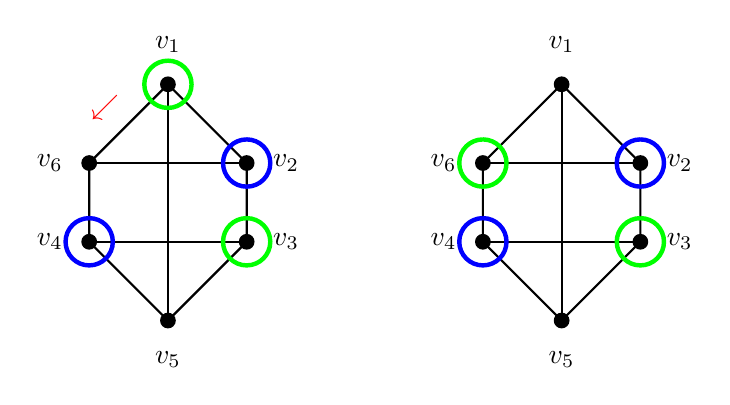
\begin{tikzpicture}[scale=1]
\def\ver{0.1} %size of a vertex
\def\xa{1}
\def\ya{5}
%---------------------Graph2------------------
%nodes
\def\xb{6}
\path[fill] (\xb,\ya) circle (\ver);       % v5
\path[fill] (\xb+1,\ya+1) circle (\ver);   % v3
\path[fill] (\xb+1,\ya+2) circle (\ver);   % v2
\path[fill] (\xb,\ya+3) circle (\ver);     % v1
\path[fill] (\xb-1,\ya+2) circle (\ver);   % v6
\path[fill] (\xb-1,\ya+1) circle (\ver);   % v4
%labels
\node (1) at (\xb,\ya+3.5) {$v_1$};     % v1
\node (2) at (\xb+1.5,\ya+2) {$v_2$};   % v2
\node (3) at (\xb+1.5,\ya+1) {$v_3$};   % v3
\node (5) at (\xb,\ya-0.5) {$v_5$};     % v5
\node (4) at (\xb-1.5,\ya+1) {$v_4$};   % v4
\node (6) at (\xb-1.5,\ya+2) {$v_6$};   % v6
%mid-slide
\node [color=red, ultra thick](7) at (5.2,7.7) {$\swarrow$};
%edges
\draw[thick] (\xb,\ya)--(\xb+1,\ya+1)--(\xb+1,\ya+2)--(\xb,\ya+3)--(\xb-1,\ya+2)--(\xb-1,\ya+1)--(\xb,\ya) ; % contour
\draw[thick] (\xb,\ya)--(\xb,\ya+3) ;       % v5 - v1
\draw[thick] (\xb+1,\ya+1)--(\xb-1,\ya+1) ; % v3 - v4
\draw[thick] (\xb+1,\ya+2)--(\xb-1,\ya+2) ; % v2 - v6
%independent sets
\draw[ultra thick,green] (\xb,\ya+3+ \ver+0.2) coordinate(a1)  arc (90:450:\ver +0.2) coordinate(a2);
\draw[ultra thick,green] (\xb+1,\ya+1+ \ver+0.2) coordinate(d1)  arc (90:450:\ver +0.2) coordinate(d2);
\draw[ultra thick,blue] (\xb-1,\ya+1+ \ver+0.2) coordinate(a1)  arc (90:450:\ver +0.2) coordinate(a2);
\draw[ultra thick,blue] (\xb+1,\ya+2+ \ver+0.2) coordinate(d1)  arc (90:450:\ver +0.2) coordinate(d2);

%---------------------Graph3-----------------------
%nodes
\def\xc{11}
\path[fill] (\xc,\ya) circle (\ver);       % v5
\path[fill] (\xc+1,\ya+1) circle (\ver);   % v3
\path[fill] (\xc+1,\ya+2) circle (\ver);   % v2
\path[fill] (\xc,\ya+3) circle (\ver);     % v1
\path[fill] (\xc-1,\ya+2) circle (\ver);   % v6
\path[fill] (\xc-1,\ya+1) circle (\ver);   % v4
%labels
\node (1) at (\xc,\ya+3.5) {$v_1$};     % v1
\node (2) at (\xc+1.5,\ya+2) {$v_2$};   % v2
\node (3) at (\xc+1.5,\ya+1) {$v_3$};   % v3
\node (5) at (\xc,\ya-0.5) {$v_5$};     % v5
\node (4) at (\xc-1.5,\ya+1) {$v_4$};   % v4
\node (6) at (\xc-1.5,\ya+2) {$v_6$};   % v6
%edges
\draw[thick] (\xc,\ya)--(\xc+1,\ya+1)--(\xc+1,\ya+2)--(\xc,\ya+3)--(\xc-1,\ya+2)--(\xc-1,\ya+1)--(\xc,\ya) ; % contour
\draw[thick] (\xc,\ya)--(\xc,\ya+3) ;       % v5 - v1
\draw[thick] (\xc+1,\ya+1)--(\xc-1,\ya+1) ; % v3 - v4
\draw[thick] (\xc+1,\ya+2)--(\xc-1,\ya+2) ; % v2 - v6
%independent sets
\draw[ultra thick,green] (\xc-1,\ya+2+ \ver+0.2) coordinate(a1)  arc (90:450:\ver +0.2) coordinate(a2);
\draw[ultra thick,green] (\xc+1,\ya+1+ \ver+0.2) coordinate(d1)  arc (90:450:\ver +0.2) coordinate(d2);
\draw[ultra thick,blue] (\xc-1,\ya+1+ \ver+0.2) coordinate(a1)  arc (90:450:\ver +0.2) coordinate(a2);
\draw[ultra thick,blue] (\xc+1,\ya+2+ \ver+0.2) coordinate(d1)  arc (90:450:\ver +0.2) coordinate(d2);
\end{tikzpicture}  }

\vspace{3em} % vertical space

\subfigure {
\begin{tikzpicture}[scale=1]
\node (1) [draw, rectangle] {$C_1 = \{ \{v_2, v_4, v_5, v_6\}, \{v_1, t_1\}, \{v_3, t_2\} \}$.};
\node (2) [below=of 1, draw, rectangle] {$C_2 = \{ \{v_1, v_2, v_4, v_5, v_6, t_1\}, \{v_3, t_2\} \}$.};
\node (3) [below=of 2, draw, rectangle] {$C_3 = \{ \{v_1, v_2, v_4, v_5\}, \{v_6, t_1\}, \{v_3, t_2\} \}$.};
\draw[->]  (1) to node [auto] {merge} (2);
\draw[->]  (2) to node [auto] {split} (3);
\end{tikzpicture} }
\end{scaletikzpicturetowidth}
\end{center}
\caption{}
\end{figure}


\begin{example}{Complete example of the reduction}
\begin{figure}[H]
\begin{center}
\begin{scaletikzpicturetowidth}{\textwidth}
\subfigure {
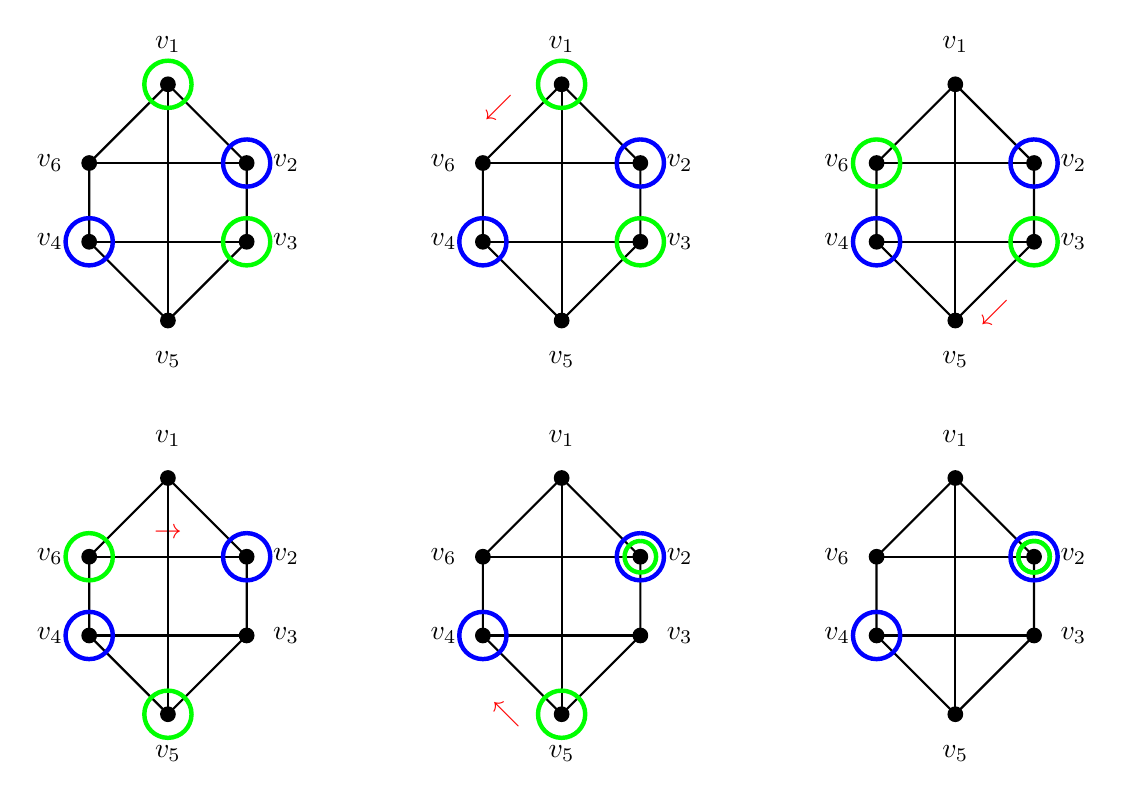
\begin{tikzpicture}[scale=1]

\def\ver{0.1} %size of a vertex
\def\xa{1}
\def\ya{5}
%--------------------- Graph 1 ---------------------
%nodes
\path[fill] (\xa,\ya) circle (\ver);       % v5
\path[fill] (\xa+1,\ya+1) circle (\ver);   % v3
\path[fill] (\xa+1,\ya+2) circle (\ver);   % v2
\path[fill] (\xa,\ya+3) circle (\ver);     % v1
\path[fill] (\xa-1,\ya+2) circle (\ver);   % v6
\path[fill] (\xa-1,\ya+1) circle (\ver);   % v4
%labels
\node (1) at (\xa,\ya+3.5) {$v_1$};     % v1
\node (2) at (\xa+1.5,\ya+2) {$v_2$};   % v2
\node (3) at (\xa+1.5,\ya+1) {$v_3$};   % v3
\node (5) at (\xa,\ya-0.5) {$v_5$};     % v5
\node (4) at (\xa-1.5,\ya+1) {$v_4$};   % v4
\node (6) at (\xa-1.5,\ya+2) {$v_6$};   % v6
%edges
\draw[thick] (\xa,\ya)--(\xa+1,\ya+1)--(\xa+1,\ya+2)--(\xa,\ya+3)--(\xa-1,\ya+2)--(\xa-1,\ya+1)--(\xa,\ya) ; % contour
\draw[thick] (\xa,\ya)--(\xa,\ya+3) ;       % v5 - v1
\draw[thick] (\xa+1,\ya+1)--(\xa-1,\ya+1) ; % v3 - v4
\draw[thick] (\xa+1,\ya+2)--(\xa-1,\ya+2) ; % v2 - v6
%independent sets
\draw[ultra thick,green] (\xa,\ya+3+ \ver+0.2) coordinate(a1)  arc (90:450:\ver +0.2) coordinate(a2);
\draw[ultra thick,green] (\xa+1,\ya+1+ \ver+0.2) coordinate(d1)  arc (90:450:\ver +0.2) coordinate(d2);
\draw[ultra thick,blue] (\xa-1,\ya+1+ \ver+0.2) coordinate(a1)  arc (90:450:\ver +0.2) coordinate(a2);
\draw[ultra thick,blue] (\xa+1,\ya+2+ \ver+0.2) coordinate(d1)  arc (90:450:\ver +0.2) coordinate(d2);


%---------------------Graph2------------------
%nodes
\def\xb{6}
\path[fill] (\xb,\ya) circle (\ver);       % v5
\path[fill] (\xb+1,\ya+1) circle (\ver);   % v3
\path[fill] (\xb+1,\ya+2) circle (\ver);   % v2
\path[fill] (\xb,\ya+3) circle (\ver);     % v1
\path[fill] (\xb-1,\ya+2) circle (\ver);   % v6
\path[fill] (\xb-1,\ya+1) circle (\ver);   % v4
%labels
\node (1) at (\xb,\ya+3.5) {$v_1$};     % v1
\node (2) at (\xb+1.5,\ya+2) {$v_2$};   % v2
\node (3) at (\xb+1.5,\ya+1) {$v_3$};   % v3
\node (5) at (\xb,\ya-0.5) {$v_5$};     % v5
\node (4) at (\xb-1.5,\ya+1) {$v_4$};   % v4
\node (6) at (\xb-1.5,\ya+2) {$v_6$};   % v6
%mid-slide
\node [color=red, ultra thick](7) at (5.2,7.7) {$\swarrow$};
%edges
\draw[thick] (\xb,\ya)--(\xb+1,\ya+1)--(\xb+1,\ya+2)--(\xb,\ya+3)--(\xb-1,\ya+2)--(\xb-1,\ya+1)--(\xb,\ya) ; % contour
\draw[thick] (\xb,\ya)--(\xb,\ya+3) ;       % v5 - v1
\draw[thick] (\xb+1,\ya+1)--(\xb-1,\ya+1) ; % v3 - v4
\draw[thick] (\xb+1,\ya+2)--(\xb-1,\ya+2) ; % v2 - v6
%independent sets
\draw[ultra thick,green] (\xb,\ya+3+ \ver+0.2) coordinate(a1)  arc (90:450:\ver +0.2) coordinate(a2);
\draw[ultra thick,green] (\xb+1,\ya+1+ \ver+0.2) coordinate(d1)  arc (90:450:\ver +0.2) coordinate(d2);
\draw[ultra thick,blue] (\xb-1,\ya+1+ \ver+0.2) coordinate(a1)  arc (90:450:\ver +0.2) coordinate(a2);
\draw[ultra thick,blue] (\xb+1,\ya+2+ \ver+0.2) coordinate(d1)  arc (90:450:\ver +0.2) coordinate(d2);

%---------------------Graph3-----------------------
%nodes
\def\xc{11}
\path[fill] (\xc,\ya) circle (\ver);       % v5
\path[fill] (\xc+1,\ya+1) circle (\ver);   % v3
\path[fill] (\xc+1,\ya+2) circle (\ver);   % v2
\path[fill] (\xc,\ya+3) circle (\ver);     % v1
\path[fill] (\xc-1,\ya+2) circle (\ver);   % v6
\path[fill] (\xc-1,\ya+1) circle (\ver);   % v4
%labels
\node (1) at (\xc,\ya+3.5) {$v_1$};     % v1
\node (2) at (\xc+1.5,\ya+2) {$v_2$};   % v2
\node (3) at (\xc+1.5,\ya+1) {$v_3$};   % v3
\node (5) at (\xc,\ya-0.5) {$v_5$};     % v5
\node (4) at (\xc-1.5,\ya+1) {$v_4$};   % v4
\node (6) at (\xc-1.5,\ya+2) {$v_6$};   % v6
%mid-slide
\node [color=red, ultra thick](7) at (\xc+0.5,\ya+0.1) {$\swarrow$};
%edges
\draw[thick] (\xc,\ya)--(\xc+1,\ya+1)--(\xc+1,\ya+2)--(\xc,\ya+3)--(\xc-1,\ya+2)--(\xc-1,\ya+1)--(\xc,\ya) ; % contour
\draw[thick] (\xc,\ya)--(\xc,\ya+3) ;       % v5 - v1
\draw[thick] (\xc+1,\ya+1)--(\xc-1,\ya+1) ; % v3 - v4
\draw[thick] (\xc+1,\ya+2)--(\xc-1,\ya+2) ; % v2 - v6
%independent sets
\draw[ultra thick,green] (\xc-1,\ya+2+ \ver+0.2) coordinate(a1)  arc (90:450:\ver +0.2) coordinate(a2);
\draw[ultra thick,green] (\xc+1,\ya+1+ \ver+0.2) coordinate(d1)  arc (90:450:\ver +0.2) coordinate(d2);
\draw[ultra thick,blue] (\xc-1,\ya+1+ \ver+0.2) coordinate(a1)  arc (90:450:\ver +0.2) coordinate(a2);
\draw[ultra thick,blue] (\xc+1,\ya+2+ \ver+0.2) coordinate(d1)  arc (90:450:\ver +0.2) coordinate(d2);

%--------------------- Graph 4 ---------------------
\def\ya{0}
%nodes
\path[fill] (\xa,\ya) circle (\ver);       % v5
\path[fill] (\xa+1,\ya+1) circle (\ver);   % v3
\path[fill] (\xa+1,\ya+2) circle (\ver);   % v2
\path[fill] (\xa,\ya+3) circle (\ver);     % v1
\path[fill] (\xa-1,\ya+2) circle (\ver);   % v6
\path[fill] (\xa-1,\ya+1) circle (\ver);   % v4
%labels
\node (1) at (\xa,\ya+3.5) {$v_1$};     % v1
\node (2) at (\xa+1.5,\ya+2) {$v_2$};   % v2
\node (3) at (\xa+1.5,\ya+1) {$v_3$};   % v3
\node (5) at (\xa,\ya-0.5) {$v_5$};     % v5
\node (4) at (\xa-1.5,\ya+1) {$v_4$};   % v4
\node (6) at (\xa-1.5,\ya+2) {$v_6$};   % v6
%mid-slide
\node [color=red, ultra thick](7) at (\xa,\ya+2.3) {$\rightarrow$};
%edges
\draw[thick] (\xa,\ya)--(\xa+1,\ya+1)--(\xa+1,\ya+2)--(\xa,\ya+3)--(\xa-1,\ya+2)--(\xa-1,\ya+1)--(\xa,\ya) ; % contour
\draw[thick] (\xa,\ya)--(\xa,\ya+3) ;       % v5 - v1
\draw[thick] (\xa+1,\ya+1)--(\xa-1,\ya+1) ; % v3 - v4
\draw[thick] (\xa+1,\ya+2)--(\xa-1,\ya+2) ; % v2 - v6
%independent sets
\draw[ultra thick,green] (\xa-1,\ya+2+ \ver+0.2) coordinate(a1)  arc (90:450:\ver +0.2) coordinate(a2); % v6
\draw[ultra thick,green] (\xa,\ya+ \ver+0.2) coordinate(d1)  arc (90:450:\ver +0.2) coordinate(d2); % v5
\draw[ultra thick,blue] (\xa-1,\ya+1+ \ver+0.2) coordinate(a1)  arc (90:450:\ver +0.2) coordinate(a2);
\draw[ultra thick,blue] (\xa+1,\ya+2+ \ver+0.2) coordinate(d1)  arc (90:450:\ver +0.2) coordinate(d2);

%---------------------Graph 5 ------------------
%nodes
\def\xb{6}
\path[fill] (\xb,\ya) circle (\ver);       % v5
\path[fill] (\xb+1,\ya+1) circle (\ver);   % v3
\path[fill] (\xb+1,\ya+2) circle (\ver);   % v2
\path[fill] (\xb,\ya+3) circle (\ver);     % v1
\path[fill] (\xb-1,\ya+2) circle (\ver);   % v6
\path[fill] (\xb-1,\ya+1) circle (\ver);   % v4
%labels
\node (1) at (\xb,\ya+3.5) {$v_1$};     % v1
\node (2) at (\xb+1.5,\ya+2) {$v_2$};   % v2
\node (3) at (\xb+1.5,\ya+1) {$v_3$};   % v3
\node (5) at (\xb,\ya-0.5) {$v_5$};     % v5
\node (4) at (\xb-1.5,\ya+1) {$v_4$};   % v4
\node (6) at (\xb-1.5,\ya+2) {$v_6$};   % v6
%mid-slide
\node [color=red, ultra thick](7) at (\xb-0.7,\ya) {$\nwarrow$};
%edges
\draw[thick] (\xb,\ya)--(\xb+1,\ya+1)--(\xb+1,\ya+2)--(\xb,\ya+3)--(\xb-1,\ya+2)--(\xb-1,\ya+1)--(\xb,\ya) ; % contour
\draw[thick] (\xb,\ya)--(\xb,\ya+3) ;       % v5 - v1
\draw[thick] (\xb+1,\ya+1)--(\xb-1,\ya+1) ; % v3 - v4
\draw[thick] (\xb+1,\ya+2)--(\xb-1,\ya+2) ; % v2 - v6
%independent sets
\draw[ultra thick,green] (\xb+1,\ya+2+ \ver+0.1) coordinate(a1)  arc (90:450:\ver +0.1) coordinate(a2);   % v4
\draw[ultra thick,green] (\xb,\ya+ \ver+0.2) coordinate(d1)  arc (90:450:\ver +0.2) coordinate(d2);       % v5
\draw[ultra thick,blue] (\xb-1,\ya+1+ \ver+0.2) coordinate(a1)  arc (90:450:\ver +0.2) coordinate(a2);    % v4
\draw[ultra thick,blue] (\xb+1,\ya+2+ \ver+0.2) coordinate(d1)  arc (90:450:\ver +0.2) coordinate(d2);    % v2

%---------------------Graph 6 -----------------------
%nodes
\def\xc{11}
\path[fill] (\xc,\ya) circle (\ver);       % v5
\path[fill] (\xc+1,\ya+1) circle (\ver);   % v3
\path[fill] (\xc+1,\ya+2) circle (\ver);   % v2
\path[fill] (\xc,\ya+3) circle (\ver);     % v1
\path[fill] (\xc-1,\ya+2) circle (\ver);   % v6
\path[fill] (\xc-1,\ya+1) circle (\ver);   % v4
%labels
\node (1) at (\xc,\ya+3.5) {$v_1$};     % v1
\node (2) at (\xc+1.5,\ya+2) {$v_2$};   % v2
\node (3) at (\xc+1.5,\ya+1) {$v_3$};   % v3
\node (5) at (\xc,\ya-0.5) {$v_5$};     % v5
\node (4) at (\xc-1.5,\ya+1) {$v_4$};   % v4
\node (6) at (\xc-1.5,\ya+2) {$v_6$};   % v6
%edges
\draw[thick] (\xc,\ya)--(\xc+1,\ya+1)--(\xc+1,\ya+2)--(\xc,\ya+3)--(\xc-1,\ya+2)--(\xc-1,\ya+1)--(\xc,\ya) ; % contour
\draw[thick] (\xc,\ya)--(\xc,\ya+3) ;       % v5 - v1
\draw[thick] (\xc+1,\ya+1)--(\xc-1,\ya+1) ; % v3 - v4
\draw[thick] (\xc+1,\ya+2)--(\xc-1,\ya+2) ; % v2 - v6
%independent sets
\draw[ultra thick,green] (\xc+1,\ya+2+ \ver+0.1) coordinate(a1)  arc (90:450:\ver +0.1) coordinate(a2);   % v4
\draw[ultra thick,green] (\xc+1,\ya+2+ \ver+0.1) coordinate(d1)  arc (90:450:\ver +0.1) coordinate(d2);   % v2
\draw[ultra thick,blue] (\xc-1,\ya+1+ \ver+0.2) coordinate(a1)  arc (90:450:\ver +0.2) coordinate(a2);    % v4
\draw[ultra thick,blue] (\xc+1,\ya+2+ \ver+0.2) coordinate(d1)  arc (90:450:\ver +0.2) coordinate(d2);    % v2

\end{tikzpicture} }

\vspace{3em} % vertical space

\subfigure {
\begin{tikzpicture}[scale=1]
\node (1) [draw, rectangle] {$C_1 = \{ \{v_2, v_4, v_5, v_6\}, \textcolor{green}{\{v_1, t_1\}}, \textcolor{green}{\{v_3, t_2\}} \}$.};
\node (2) [below right=of 1, draw, rectangle] {$C_2 = \{ \{v_1, v_2, v_4, v_5, v_6, \textcolor{red}{t_1}\}, \textcolor{green}{\{v_3, t_2\}} \}$.};
\node (3) [below left=of 2, draw, rectangle] {$C_3 = \{ \{v_1, v_2, v_4, v_5\}, \textcolor{green}{\{v_6, t_1\}}, \textcolor{green}{\{v_3, t_2\}} \}$.};
\node (4) [below right=of 3, draw, rectangle] {$C_4 = \{ \{v_1, v_2, v_3, v_4, v_5, \textcolor{red}{t_2}\}, \textcolor{green}{\{v_6, t_1\}} \}$.};
\node (5) [below left=of 4, draw, rectangle] {$C_5 = \{ \{v_1, v_2, v_3, v_4\}, \textcolor{green}{\{v_5, t_2\}}, \textcolor{green}{\{v_6, t_1\}} \}$.};
\node (6) [below right=of 5, draw, rectangle] {$C_6 = \{ \{v_1, v_2, v_3, v_4,v_6,\textcolor{red}{t_1}\}, \textcolor{green}{\{v_5, t_2\}} \}$.};
\node (7) [below left=of 6, draw, rectangle] {$C_7 = \{ \{v_1, v_3, v_4,v_6\}, \textcolor{green}{\{v_2, t_1\}}, \textcolor{green}{\{v_5, t_2\}}\}$.};
\node (8) [below right=of 7, draw, rectangle] {$C_8 = \{ \{v_1, v_3, v_4, v_5, v_6, \textcolor{red}{t_2}\}, \textcolor{green}{\{v_2, t_1\}} \}$.};
\node (9) [below left=of 8, draw, rectangle] {$C_9 = \{ \{v_1, v_3, v_5, v_6\}, \textcolor{blue}{\{v_2, t_1\}}, \textcolor{blue}{\{v_4, t_2\}} \}$.};
\draw[->]  (1) to node [auto] {merge} (2);
\draw[->]  (2) to node [auto] {split} (3);
\draw[->]  (3) to node [auto] {merge} (4);
\draw[->]  (4) to node [auto] {split} (5);
\draw[->]  (5) to node [auto] {merge} (6);
\draw[->]  (6) to node [auto] {split} (7);
\draw[->]  (7) to node [auto] {merge} (8);
\draw[->]  (8) to node [auto] {split} (9);
\end{tikzpicture} }
\end{scaletikzpicturetowidth}
\end{scaletikzpicturetowidth}
\end{center}
\caption{}
\end{figure}
\end{example}



%%%%%%%%%%%%%%%%%%%%%%%%%%%%%%%%%%%%%%%% BEGINING OF A FIGURE : All possible moves of an AND vertex %%%%%%%%%%%%%%%%%%%%%%%%%%%%%%%%%%%%%%%%%%%
\begin{figure}[H]
\begin{center}
\begin{scaletikzpicturetowidth}{\textwidth}
\begin{tikzpicture}[scale=0.7]
% v1
\def\xa{0}
\def\ya{0}
% v2
\def\xb{\xa-3}
\def\yb{\ya+3}
% v3
\def\xc{\xa+3}
\def\yc{\ya+3}
% v4
\def\xd{\xa}
\def\yd{\ya+6}
% v5
\def\xe{\xa}
\def\ye{\ya-4}
%labels
\node (1) at (\xa+2,\ya) {$f_1$};
\node (2) at (\xb-2,\yb) {$f_2$};
\node (3) at (\xc+2,\yc) {$f_3$};
\node (5) at (\xd+2,\yd) {$f_4$};
\node (4) at (\xe+2,\ye) {$f_0$};
% f_1 arrows
\draw[middlearrow={<}, red] (\xa, \ya) -- (\xa+0.9, \ya-0.8);
\draw[middlearrow={<}, red] (\xa, \ya) -- (\xa-1, \ya-0.8);
\draw[middlearrow={<}, blue] (\xa, \ya) -- (\xa, \ya+1);
\draw[ultra thick, -, blue] (\xa, \ya) -- (\xa, \ya+1);
\draw[ultra thick, -, red] (\xa, \ya) -- (\xa+0.9, \ya-0.8);
\draw[ultra thick, -, red] (\xa, \ya) -- (\xa-1, \ya-0.8);
\path[fill=none, draw, ultra thick, dotted] (\xa,\ya) circle (\ver+1.2);     %f1
% f_2 arrows
\draw[middlearrow={>}, red] (\xb, \yb) --(\xb-0.9, \yb-0.8);
\draw[middlearrow={<}, red] (\xb, \yb) --(\xb+0.9, \yb-0.8);
\draw[middlearrow={<}, blue] (\xb, \yb) --(\xb, \yb+1);
\draw[ultra thick, -, red] (\xb, \yb) --(\xb-0.9, \yb-0.8);
\draw[ultra thick, -, red] (\xb, \yb) --(\xb+0.9, \yb-0.8);
\draw[ultra thick, -, blue] (\xb, \yb) --(\xb, \yb+1);
\path[fill=none, draw, ultra thick, dotted] (\xb,\yb) circle (\ver+1.2);     %f2
% f_3  arrows
\draw[middlearrow={<}, red] (\xc, \yc) --(\xc-0.9, \yc-0.8);
\draw[middlearrow={>}, red] (\xc, \yc) --(\xc+0.9, \yc-0.8);
\draw[middlearrow={<}, blue] (\xc, \yc) --(\xc, \yc+1);
\draw[ultra thick, -, red] (\xc, \yc) --(\xc-0.9, \yc-0.8);
\draw[ultra thick, -, red] (\xc, \yc) --(\xc+0.9, \yc-0.8);
\draw[ultra thick, -, blue] (\xc, \yc) --(\xc, \yc+1);
\path[fill=none, draw, ultra thick, dotted] (\xc,\yc) circle (\ver+1.2);     %f3
% f_4  arrows
\draw[middlearrow={>}, red] (\xd, \yd) --(\xd-0.9, \yd-0.8);
\draw[middlearrow={>}, red] (\xd, \yd) --(\xd+0.9, \yd-0.8);
\draw[middlearrow={<}, blue] (\xd, \yd) --(\xd, \yd+1);
\draw[ultra thick, -, red] (\xd, \yd) --(\xd-0.9, \yd-0.8);
\draw[ultra thick, -, red] (\xd, \yd) --(\xd+0.9, \yd-0.8);
\draw[ultra thick, -, blue] (\xd, \yd) --(\xd, \yd+1);
\path[fill=none, draw, ultra thick, dotted] (\xd,\yd) circle (\ver+1.2);     %f4
% f_0  arrows
\draw[middlearrow={<}, red] (\xe, \ye) --(\xe-0.9, \ye-0.8);
\draw[middlearrow={<}, red] (\xe, \ye) --(\xe+0.9, \ye-0.8);
\draw[middlearrow={>}, blue] (\xe, \ye) --(\xe, \ye+1);
\draw[ultra thick, -, red] (\xe, \ye) --(\xe-0.9, \ye-0.8);
\draw[ultra thick, -, red] (\xe, \ye) --(\xe+0.9, \ye-0.8);
\draw[ultra thick, -, blue] (\xe, \ye) --(\xe, \ye+1);
\path[fill=none, draw, ultra thick, dotted] (\xe,\ye) circle (\ver+1.2);     %f0
%relations
\draw[ultra thick, <->] (\xe,\ye+1.4) -- (\xa,\ya-1.4);
\draw[ultra thick, <->] (\xa+1,\ya+1) -- (\xc-1,\yc-1);
\draw[ultra thick, <->] (\xa-1,\ya+1) -- (\xb+1,\yb-1);
\draw[ultra thick, <->] (\xc-1,\yc+1) -- (\xd+1,\yd-1);
\draw[ultra thick, <->] (\xd-1,\yd-1) -- (\xb+1,\yb+1);
%graph G : Nodes fill
\path[fill] (\xa,\ya) circle (\ver);     %f1
\path[fill] (\xb,\yb) circle (\ver);     %f2
\path[fill] (\xc,\yc) circle (\ver);     %f3
\path[fill] (\xd,\yd) circle (\ver);     %f4
\path[fill] (\xe,\ye) circle (\ver);     %f0
\end{tikzpicture}
\end{scaletikzpicturetowidth}
\end{center}
\caption{All the possible orientations of edges of an AND vertex.}
\label{fig:and_all_possible_moves}
\end{figure}
%%%%%%%%%%%%%%%%%%%%%%%%%%%%%%%%%%%%%%%%%%% ENDING OF A FIGURE %%%%%%%%%%%%%%%%%%%%%%%%%%%%%%%%%%%%%%%

%%%%%%%%%%%%%%%%%%%%%%%%%%%%%%%%%%%%%% BEGINING OF A FIGURE : All possible moves of an OR vertex  %%%%%%%%%%%%%%%%%%%%%%%%%%%%%%%%%%%%%
\begin{figure}[H]
\begin{center}
\begin{scaletikzpicturetowidth}{\textwidth}
\begin{tikzpicture}[scale=0.7]
% v1
\def\xa{0}
\def\ya{0}
% v2
\def\xb{\xa-3}
\def\yb{\ya+3}
% v3
\def\xc{\xa+3}
\def\yc{\ya+3}
% v4
\def\xd{\xa}
\def\yd{\ya+6}
% v5
\def\xe{\xa}
\def\ye{\ya-4}
% v6
\def\xf{\xa-3}
\def\yf{\ya-7}
% v7
\def\xg{\xa+3}
\def\yg{\ya-7}
%labels
\node (1) at (\xa+2,\ya) {$f_1$};
\node (2) at (\xb-2,\yb) {$f_2$};
\node (3) at (\xc+2,\yc) {$f_3$};
\node (5) at (\xd+2,\yd) {$f_4$};
\node (4) at (\xe+2,\ye) {$f_0$};
\node (6) at (\xf-2,\yf) {$f_6$};
\node (7) at (\xg+2,\yg) {$f_7$};
% f_1 arrows
\draw[middlearrow={<}, blue] (\xa, \ya) -- (\xa+0.9, \ya-0.8);
\draw[middlearrow={<}, blue] (\xa, \ya) -- (\xa-1, \ya-0.8);
\draw[middlearrow={<}, blue] (\xa, \ya) -- (\xa, \ya+1);
\draw[ultra thick, -, blue] (\xa, \ya) -- (\xa, \ya+1);
\draw[ultra thick, -, blue] (\xa, \ya) -- (\xa+0.9, \ya-0.8);
\draw[ultra thick, -, blue] (\xa, \ya) -- (\xa-1, \ya-0.8);
\path[fill=none, draw, ultra thick, dotted] (\xa,\ya) circle (\ver+1.2);     %f1
% f_2 arrows
\draw[middlearrow={>}, blue] (\xb, \yb) --(\xb-0.9, \yb-0.8);
\draw[middlearrow={<}, blue] (\xb, \yb) --(\xb+0.9, \yb-0.8);
\draw[middlearrow={<}, blue] (\xb, \yb) --(\xb, \yb+1);
\draw[ultra thick, -, blue] (\xb, \yb) --(\xb-0.9, \yb-0.8);
\draw[ultra thick, -, blue] (\xb, \yb) --(\xb+0.9, \yb-0.8);
\draw[ultra thick, -, blue] (\xb, \yb) --(\xb, \yb+1);
\path[fill=none, draw, ultra thick, dotted] (\xb,\yb) circle (\ver+1.2);     %f2
% f_3  arrows
\draw[middlearrow={<}, blue] (\xc, \yc) --(\xc-0.9, \yc-0.8);
\draw[middlearrow={>}, blue] (\xc, \yc) --(\xc+0.9, \yc-0.8);
\draw[middlearrow={<}, blue] (\xc, \yc) --(\xc, \yc+1);
\draw[ultra thick, -, blue] (\xc, \yc) --(\xc-0.9, \yc-0.8);
\draw[ultra thick, -, blue] (\xc, \yc) --(\xc+0.9, \yc-0.8);
\draw[ultra thick, -, blue] (\xc, \yc) --(\xc, \yc+1);
\path[fill=none, draw, ultra thick, dotted] (\xc,\yc) circle (\ver+1.2);     %f3
% f_4  arrows
\draw[middlearrow={>}, blue] (\xd, \yd) --(\xd-0.9, \yd-0.8);
\draw[middlearrow={>}, blue] (\xd, \yd) --(\xd+0.9, \yd-0.8);
\draw[middlearrow={<}, blue] (\xd, \yd) --(\xd, \yd+1);
\draw[ultra thick, -, blue] (\xd, \yd) --(\xd-0.9, \yd-0.8);
\draw[ultra thick, -, blue] (\xd, \yd) --(\xd+0.9, \yd-0.8);
\draw[ultra thick, -, blue] (\xd, \yd) --(\xd, \yd+1);
\path[fill=none, draw, ultra thick, dotted] (\xd,\yd) circle (\ver+1.2);     %f4
% f_0  arrows
\draw[middlearrow={<}, blue] (\xe, \ye) --(\xe-0.9, \ye-0.8);
\draw[middlearrow={<}, blue] (\xe, \ye) --(\xe+0.9, \ye-0.8);
\draw[middlearrow={>}, blue] (\xe, \ye) --(\xe, \ye+1);
\draw[ultra thick, -, blue] (\xe, \ye) --(\xe-0.9, \ye-0.8);
\draw[ultra thick, -, blue] (\xe, \ye) --(\xe+0.9, \ye-0.8);
\draw[ultra thick, -, blue] (\xe, \ye) --(\xe, \ye+1);
\path[fill=none, draw, ultra thick, dotted] (\xe,\ye) circle (\ver+1.2);     %f0
% f_6 arrows
\draw[middlearrow={>}, blue] (\xf, \yf) --(\xf-0.9, \yf-0.8);
\draw[middlearrow={<}, blue] (\xf, \yf) --(\xf+0.9, \yf-0.8);
\draw[middlearrow={>}, blue] (\xf, \yf) --(\xf, \yf+1);
\draw[ultra thick, -, blue] (\xf, \yf) --(\xf-0.9, \yf-0.8);
\draw[ultra thick, -, blue] (\xf, \yf) --(\xf+0.9, \yf-0.8);
\draw[ultra thick, -, blue] (\xf, \yf) --(\xf, \yf+1);
\path[fill=none, draw, ultra thick, dotted] (\xf,\yf) circle (\ver+1.2);     %f6
% f_7 arrows
\draw[middlearrow={<}, blue] (\xg, \yg) --(\xg-0.9, \yg-0.8);
\draw[middlearrow={>}, blue] (\xg, \yg) --(\xg+0.9, \yg-0.8);
\draw[middlearrow={>}, blue] (\xg, \yg) --(\xg, \yg+1);
\draw[ultra thick, -, blue] (\xg, \yg) --(\xg-0.9, \yg-0.8);
\draw[ultra thick, -, blue] (\xg, \yg) --(\xg+0.9, \yg-0.8);
\draw[ultra thick, -, blue] (\xg, \yg) --(\xg, \yg+1);
\path[fill=none, draw, ultra thick, dotted] (\xg,\yg) circle (\ver+1.2);     %f7
%relations
\draw[ultra thick, <->] (\xe,\ye+1.4) -- (\xa,\ya-1.4);
\draw[ultra thick, <->] (\xa+1,\ya+1) -- (\xc-1,\yc-1);
\draw[ultra thick, <->] (\xa-1,\ya+1) -- (\xb+1,\yb-1);
\draw[ultra thick, <->] (\xc-1,\yc+1) -- (\xd+1,\yd-1);
\draw[ultra thick, <->] (\xd-1,\yd-1) -- (\xb+1,\yb+1);
\draw[ultra thick, <->] (\xe-1,\ye-1) -- (\xf+1,\yf+1);
\draw[ultra thick, <->] (\xe+1,\ye-1) -- (\xg-1,\yg+1);
%graph G : Nodes fill
\path[fill] (\xa,\ya) circle (\ver);     %f1
\path[fill] (\xb,\yb) circle (\ver);     %f2
\path[fill] (\xc,\yc) circle (\ver);     %f3
\path[fill] (\xd,\yd) circle (\ver);     %f4
\path[fill] (\xe,\ye) circle (\ver);     %f0
\path[fill] (\xf,\yf) circle (\ver);     %f6
\path[fill] (\xg,\yg) circle (\ver);     %f7
\end{tikzpicture}
\end{scaletikzpicturetowidth}
\end{center}
\caption{All the possible orientations of edges of an OR vertex.}
\label{fig:or_all_possible_moves}
\end{figure}
%%%%%%%%%%%%%%%%%%%%%%%%%%%%%%%%%%%%%%%%%%%%%%%% ENDING OF A FIGURE %%%%%%%%%%%%%%%%%%%%%%%%%%%%%%%%%%%%%%%%%%%%%%%%